This chapter provides essential background to understand of the thesis content and objectives.
It begins by introducing the graph data structure, which is crucial for comprehending Graph Neural Networks.
Additionally, the chapter provides an introduction to Graph Neural Networks, outlining their capabilities and exploring various applications.
Furthermore, it introduces two essential tools, SODA and Bambu, which are integral parts of the SODA Toolchain that served as the foundation for this research.

\section{Graphs}
\label{sec:graphs}%

\textit{Graphs} are data structures representing a collection of objects, known as vertices or nodes, and a set of edges connecting them~\cite{DBLP:journals/corr/abs-1812-08434}.
In a graph, the edges can be either directed or undirected, as shown in Figure~\ref{fig:directed_vs_undirected}, and they typically connect two vertices, which may or may not be distinct.
The vertices represent entities or elements, and the edges represent their relationships or connections.

\begin{figure}[b]
    \centering
    \subfloat[Directed Graph\label{fig:directed_graph}]{
        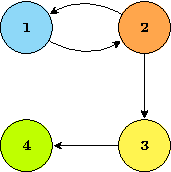
\includegraphics[height=0.2\textwidth]{Images/directed_graph}
    }
    %\quad
    \hspace{0.15\textwidth}
    \subfloat[Undirected Graph\label{fig:undirected_graph}]{
        \captionsetup{width=.4\textwidth}
        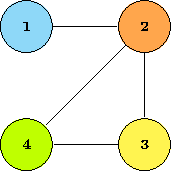
\includegraphics[height=0.2\textwidth]{Images/undirected_graph}
    }
    %\caption[Shorter caption]{This is a very long caption you don't want to appear in the List of Figures.}
    \caption{Example of directed and undirected graphs}
    \label{fig:directed_vs_undirected}
\end{figure}

Graphs serve as a versatile tool for describing diverse forms of data.
For example, molecules, the fundamental units of matter, are composed of atoms and electrons arranged in three-dimensional space.
In this intricate structure, all particles interact with each other.
However, when a pair of atoms are stably positioned at a specific distance, we refer to their connection as a covalent bond.
These bonds with distinct atomic distances can vary in nature, such as single or double bonds.
Representing this complex three-dimensional object as a graph offers a practical and widely adopted abstraction, where atoms are nodes and covalent bonds act as edges~\cite{DBLP:journals/corr/DuvenaudMAGHAA15}.

Social networks provide another domain where graphs are used: in fact, they serve as valuable tools for examining patterns within the collective behavior of people, institutions, and organizations.
By representing individuals as nodes and their relationships as edges, we can construct a graph that effectively captures groups of people and their interconnectedness.

\subsection{Graph Representation}
\label{subsec:graph_representation}

Graphs are easy to visualize, but a more formal way is needed when implementing graph algorithms.

\textbf{Adjacency matrix} \newline
The adjacency matrix of a graph is a fundamental representation that provides information about the relationships between nodes in the graph.
It provides a compact and easily interpretable representation of the graph's edges and connections, which can be easily implemented in almost all programming languages using two-dimensional arrays.

The adjacency matrix of a graph is a matrix of dimensions $N \times N$ where $N$ is the number of nodes in the graph.
Each matrix cell is set to 1 if the two nodes are connected, i.e.\ if there is an edge starting from the node of the corresponding row to the one of the corresponding column, and zero otherwise.
If the graph is undirected, each edge is bidirectional and so the matrix is symmetric.
If in the graph there are no self-loops, then the main diagonal of the matrix will be with all zeros.
Figure~\ref{fig:graph_adjacency} shows a directed graph and its adjacency matrix.

\begin{figure}[t]
    \centering
    \subfloat[Graph\label{fig:graph_example}]{
        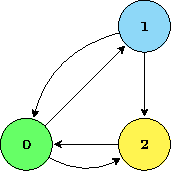
\includegraphics[height=0.2\textwidth]{Images/graph_example}
    }
    %\quad
    \hspace{0.15\textwidth}
    \subfloat[Adjacency matrix\label{fig:adjacency_mat}]{
        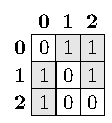
\includegraphics[height=0.2\textwidth]{Images/adjacency_matrix}
    }
    \caption{Example of a graph and its adjacency matrix}
    \label{fig:graph_adjacency}
\end{figure}

The adjacency matrix consists only of ones and zeros.
In real-world graph-related problems, the number of edges is usually much slower than the number of nodes, leading to an adjacency matrix with many zero elements.
Such matrices with mostly zero elements are called sparse matrices.
Their sparsity enables more efficient storage and manipulation, avoiding both the storage of zeros and the operations including zero elements, reducing the computational phase.

There are two common representations for sparse matrices: the Coordinate List (COO) format and the Compressed Sparse Row (CSR) format, which are explained below.

\begin{figure}[t]
    \centering
    \subfloat[COO format\label{fig:coo}]{
        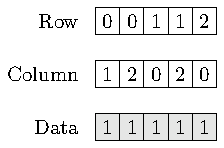
\includegraphics[height=0.2\textwidth]{Images/coo}
    }
    %\quad
    \hspace{0.15\textwidth}
    \subfloat[CSR format\label{fig:csr}]{
        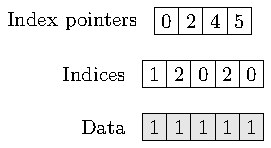
\includegraphics[height=0.2\textwidth]{Images/csr}
    }
    \caption{COO and CSR format of Adjacency matrix in Figure~\ref{fig:graph_adjacency}}
    \label{fig:coo_csr}
\end{figure}

\textbf{Coordinate format} \newline
In the COO format, a sparse matrix is represented as a list of [row, column, data] tuples, where each tuple corresponds to a non-zero element in the matrix.
The [row, column] coordinates represent the position of the non-zero element, and the value is the actual numerical value of that element.
Usually, it is preferred to store the entries first by row index and then by column index, to improve random access times.
In Figure~\ref{fig:coo_csr} the COO format of the adjacency matrix represented in Figure~\ref{fig:graph_adjacency} is reported.
For example, by considering the first element of the three arrays, it is possible to understand that the data one is placed in position [0, 1] of the adjacency matrix.

The COO format is helpful for matrices with relatively few non-zero elements because it does not require any assumptions about the sparsity pattern and allows for efficient deletion and insertion of elements.
However, it may not be the most efficient format for large and highly sparse matrices, as it may require more memory and may not support efficient row-wise or column-wise operations.
In these cases, other formats, like the CSR one, are often preferred.

\textbf{Compressed Sparse Row format} \newline
In the CSR format, a sparse matrix is represented using three arrays: the values array, the row pointers array (indices), and the column indices array (index pointers).
The data array contains the non-zero elements of the sparse matrix stored in row-major order, the array indices contains the column position of each data, while the index pointers
contains an increasing number of how many non-zero elements there are in the matrix row by row.
Given a matrix of size $m \times n$, with $NNZ$ being the number of non-zero elements, the arrays data and indices are of length $NNZ$, while the array index pointers is of length $m+1$.
Figure~\ref{fig:csr} shows the CSR format of the adjacency matrix represented in Figure~\ref{fig:graph_adjacency} is reported.

\textbf{Feature matrix} \newline
Suppose to have a graph of a social network, where each node corresponds to a person and each edge to a friendship on the social media between the two nodes.
If the aim is to predict the possible future friendship that could be established, maybe putting those people in the suggested friend list, having more information (features) about each node, such as the age or the gender, is helpful.

A feature vector represents the features or attributes associated with a single entity.
The feature matrix of a graph contains multiple feature vectors; it represents the features or attributes associated with each node.
It is commonly denoted as $X$ and  each row corresponds to a node in the graph, and each column corresponds to a specific feature or attribute of that node.

\section{Graph Neural Networks}
\label{sec:graph_neural_networks}%

%TODO: add an example image of a GNN

Graph neural networks (GNNs) are deep learning techniques that operate on graph-structured data.
Thanks to their impressive performance, GNNs have recently gained significant popularity as a widely adopted method for graph analysis~\cite{KERAMATFAR2022100401}.
Figure~\ref{fig:google_scholar} illustrates the steady growth in the number of publications related to Graph Neural Networks (GNNs) on Google Scholar from 2015 to 2022.
The data were collected by querying papers containing the specific words "Graph Neural Network" in their whole content and aggregating them on a yearly basis.
The increasing trend reflects the rising interest and research activity in the field of GNNs over the years.

\begin{figure}[t]
    \centering
    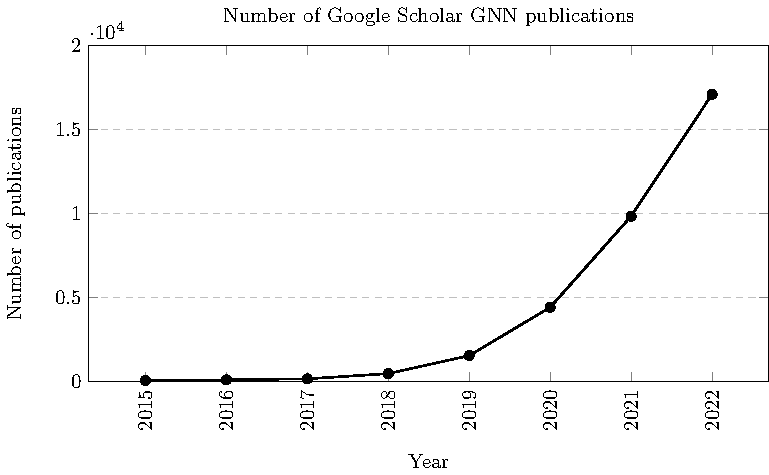
\includegraphics[width=0.7\textwidth]{Images/google_scholar}
    %\caption[Shorter caption]{This is a very long caption you don't want to appear in the List of Figures.}
    \caption{Number of GNN publications on Google Scholar per year}
    \label{fig:google_scholar}
\end{figure}

Graph Neural Networks are a group of neural networks which are designed to solve different tasks.
Prediction tasks on graphs can generally be classified into three categories: graph-level, node-level, and edge-level predictions~\cite{sanchez-lengeling2021a}.

In a graph-level task, the objective is to predict the property or characteristic of an entire graph.
For instance, when considering a molecule represented as a graph, attributes might be aimed to be predicted such as its likelihood of binding to a receptor associated with a specific disease.
This assignment is comparable to image classification tasks, where the objective is to assign a label to an entire image.
Similarly, in text analysis, sentiment analysis serves as a similar problem where the goal is to determine a complete sentence's overall mood or emotion in one go.

Node-level tasks involve predicting the identity or function of individual nodes within a graph.
One example of a node-level task is node classification in a social network.
Given a social network graph where nodes represent individuals and edges represent relationships between them, the task is to predict the demographic attributes or characteristics (e.g., age, gender, occupation) of each node based on their connection patterns and features.
Drawing an analogy to image processing, node-level prediction problems can be compared to image segmentation tasks, where the objective is to assign labels to each pixel in an image based on its role.
Similarly, in text analysis, a comparable task would involve predicting the parts of speech for each word in a sentence, such as identifying whether a word is a noun, verb, adverb, and so on.

The remaining prediction task in graphs pertains to edge prediction.
One example of an edge-level task is link prediction in a social network.
Given a graph representing a social network where, as before, in node-level tasks, nodes correspond to individuals and edges represent relationships between them, the edge-level task aims to predict missing or potential connections between nodes.
This can involve predicting the likelihood of a future friendship or the probability of a collaboration between individuals based on their shared characteristics or mutual connections in the network.

Graph Neural Networks (GNNs) are designed to process graph data and consist of multiple interconnected layers.
At its core, a GNN is an algorithm that exploits the connectivity within a graph to understand and represent the relationships between nodes.
By relying on the graph's structure, the GNN iteratively processes input edge, vertex, and graph feature vectors, which encode known attributes and transforms them into output feature vectors that capture the desired predictions.
Each Graph Neural Network typically encompasses three main stages: pre-processing, iterative updates and decoding or readout~\cite{DBLP:journals/corr/abs-2010-00130}.
\begin{enumerate}
    \item \textbf{Pre-processing}: this initial step, while optional, involves transforming the input feature vectors and graph structure representation through a pre-processing procedure.
    \item \textbf{Iterative updates}: following pre-processing, the feature vectors of each edge and vertex undergo iterative updates using aggregate-combine functions.
          For edge updates, attributes from the edge itself, connected vertices, and the graph are aggregated and combined to generate a new edge feature vector.
          Similarly, vertex updates involve aggregating feature vectors from neighboring vertices $\mathcal{N}(v)$ and combining them to obtain a new feature vector.
          This iterative process gradually incorporates relationships between increasingly distant nodes and edges, allowing for multi-hop updates.
          Furthermore, the graph may coarsen through pooling~\cite{DBLP:journals/corr/abs-1806-08804} (i.e. selective reduction or adjustment of either the graph structure or the neighborhood set of each node) in each subsequent layer, or the neighborhood set may change via layer sampling~\cite{DBLP:journals/corr/HamiltonYL17} (i.e. coarsening the graph from one layer to the next, leading to a reduction in the number of nodes that need to be processed during aggregation and combination steps).
    \item \textbf{Decoding or readout}: once the graph possesses a global feature vector, it is updated once upon completion of edge and node updates.
          The final output can be an edge/node embedding, representing specific information about each edge or node in a low-dimensional feature vector format, or a graph embedding that summarizes the entire output graph.
\end{enumerate}
Performing these stages on large and sparse graphs can introduce dynamic computational data flow and numerous irregular memory access patterns.

GNNs, as previously said, are structured into layers, each representing an iteration in the update process described earlier.
This layering allows information to propagate across nodes, enabling the influence of distant nodes.
Consequently, the appropriate number of layers in a GNN will vary depending on the significance of relationships among distant nodes in a specific application.
The commonly adopted range for the number of GNN layers is 1 to 5, as an excessive number of layers can introduce undesired problems such as feature over-smoothing, vanishing gradients, or over-fitting~\cite{DBLP:journals/corr/abs-1801-07606}.

Different popular Graph Neural Network architectures have been proposed recently, some of which are more suitable for some tasks than others.
A summary of two types of GNNs is provided in the following subsections.

\subsection{Graph Convolutional Network}
\label{subsec:graph_convolutional_network}%

A graph convolutional network (GCN)~\cite{DBLP:journals/corr/KipfW16, daigavane2021understanding} is a type of neural network architecture explicitly designed to operate on graph-structured data.
GCNs aim to learn node representations by aggregating and combining information from neighboring nodes in the graph.
The core idea behind GCNs is to perform convolution-like operations on the graph, where the convolutional filters are defined based on the graph's adjacency matrix or other graph-specific structures.
This enables GCNs to capture and leverage the structural information encoded in the graph to make predictions or perform downstream tasks.
GCNs have demonstrated effectiveness in various applications, including node classification, link prediction, and graph classification.

Given an undirected graph $\mathcal{G} = (V, E)$, where $V$ represents the set of nodes (vertices), and $E$ represents the set of edges, with an adjacency matrix $\tilde{A}=A+I_N$, where $I_N$ is the identity matrix, the layer-wise propagation rule in a GCN can be expressed as:
\begin{equation}
    \label{eq:gcn_convolution}
    H^{(l+1)} = f \left( \tilde{D}^{-\tfrac{1}{2}}  \tilde{A}  \tilde{D}^{-\tfrac{1}{2}}  H^{(l)}  W^{(l)} \right)
\end{equation}

Where $H^{(l)} \in \mathbb{R}^{N \times D}$ is the input node features matrix, $W^{(l)}$ is a layer-specific learnable weight matrix, $\tilde{D}$ is the degree matrix defined as $\tilde{D}_{ii} = \sum_{j} \tilde{A}_{ij}$, and $f(\cdot)$ represents a non-linear activation function applied element-wise, such as $ReLU(\cdot) = max(0, \cdot)$.
The equation above demonstrates the propagation of node features through graph convolution, where the adjacency matrix $\tilde{A}$ captures the connectivity information of the graph, $\tilde{D}^{-\tfrac{1}{2}}$ normalizes the adjacency matrix, and $H^{(l)}  W^{(l)}$ performs a linear transformation of node features.
The resulting $H^{(l+1)}$ represents the updated node representations after the graph convolution operation.
In practice, multiple graph convolutional layers can be stacked to capture increasingly complex relationships and further refine the node representations.

\subsection{Graph Isomorphism Network}
\label{subsec:graph_isomorphism_network}%

A Graph Isomorphism Network (GIN)~\cite{xu2019powerful, daigavane2021understanding} is a type of neural network architecture designed to operate on graph-structured data by capturing graph isomorphism, which is the property of two graphs having the same structure, inspired by the Weisfeiler-Lehman (WL) graph isomorphism test~\cite{xu2019powerful}.
GINs aim to learn node representations that are invariant under graph isomorphism, enabling them to generalize across different graphs with similar structures.

The learned vertex features from GIN-Conv can be directly utilized for tasks such as node classification and link prediction.
The model is based on the following rule:
\begin{equation}
    \label{eq:gin_function}
    h_v^{(k+1)} = MLP^{(k)} \left( \left( 1 + \epsilon^{(k)} \right) \cdot h_v^{(k)} + \sum_{u \in \mathcal{N}(v)} h_u^{(k)} \right)
\end{equation}

Where $h_v^{(k)}$ represents the initial node representation of node $v$, $\mathcal{N}(v)$ represents the neighborhood of node $v$, $\epsilon$ is a learnable
parameter or a fixed scalar, $MLP( \cdot )$ represents a Multi Layer Perceptron and $h_v^{(k+1)}$ represents the updated node representations.

In the neighborhood aggregation process of GINs, each node's representation is updated by considering its own representation and its neighbors' representations.
The neighborhood aggregation is performed through the MLP operation, followed by non-linear activation.

GINs are trained using graph-level objectives, such as graph classification or property prediction, and aim to learn invariant representations under graph isomorphism, allowing them to generalize well to unseen graphs with similar structures.
However, even if the node embeddings acquired through GIN can be directly applied to tasks such as node classification and link prediction, in the case of graph classification tasks, it is necessary to use a Readout function that takes individual node embeddings as input and produces the embedding representation for the entire graph.

The Readout function is then utilized to generate the overall representation of the graph, leveraging the individual vertex representations.
By concatenating the results from all iterations of GINConv, the final graph representation is obtained as:
\begin{equation}
    \label{eq:gin_readout}
    h_G = CONCAT \left( READOUT \left( \left\{ h_v^{(k)} | v \in G \right\} \right) | k = 0, 1, ..., K \right)
\end{equation}

Where $READOUT$ in~\ref{eq:gin_function} can be replaced with a sum operator in order to generalize the WL test~\cite{xu2019powerful}.


\section{SODA Toolchain}
\label{sec:soda}%

SODA~\cite{9786533} is a software-defined accelerator synthesizer.
It enables the creation of highly specialized accelerators from algorithms designed in high-level programming frameworks.
The synthesizer comprises a compiler-based frontend that interfaces with high-level programming frameworks, applying advanced optimizations.
It also includes a compiler-based backend responsible for generating Verilog code and interfacing with external tools to compile the final design, which can be applied to application-specific integrated circuits (ASICs) or field-programmable gate arrays (FPGAs).

SODA's exceptional power lies in its ability to offer a fully automated end-to-end hardware compiler, eliminating the need for human intervention and any modifications to the input code.
This framework seamlessly integrates with high-level Python frameworks by accepting their input descriptions, which are then translated by the frontend into a high-level intermediate representation (IR).
Leveraging the multi-level intermediate representation (MLIR), the frontend facilitates hardware/software partitioning of algorithm specifications and performs architecture-independent optimizations.
Following this, it generates a low-level IR (LLVM IR) that is utilized by the hardware generation engine, PandA-Bambu~\cite{9586110}.
PandA-Bambu can accept LLVM IR as input, making it a cutting-edge open-source HLS tool.
Throughout the entire SODA toolchain, compiler passes are employed to implement optimizations at all levels, greatly influencing the generated hardware designs' performance, area, and power characteristics.

\subsection{SODA-OPT Frontend}
\label{subsec:soda_frontend}%

SODA-OPT, the high-level compiler frontend of the SODA synthesizer, performs search, outlining, optimization, dispatching, and acceleration passes on the input program.
Its primary objective is to prepare the program for hardware synthesis, targeting either FPGAs or ASICs.
To accomplish these tasks, SODA-OPT relies on and extends the MLIR framework.
MLIR is a framework that facilitates the development of reusable, extensible, and modular compiler infrastructure by defining dialects.
These dialects serve as self-contained intermediate representations (IRs) that adhere to the meta-IR syntax of MLIR.
By utilizing dialects, code can be modeled at different levels of abstraction, allowing for specialized representations that aid in specific compiler optimizations.

 Code regions selected for hardware acceleration undergo an optimization pipeline that progressively lowers them through various MLIR dialects until they are ultimately translated into an LLVM IR format tailored explicitly for hardware synthesis.
On the other hand, the host module is lowered into an LLVM IR file containing runtime calls to control the generated custom accelerators.

\subsection{SODA Synthesizer Backend}
\label{subsec:soda_backend}%

Bambu, the SODA synthesizer backend, harnesses cutting-edge HLS techniques to produce accelerator designs using the low-level LLVM IR generated by the SODA frontend.
Bambu supports multiple frontends based on standard compilers such as GCC or CLANG.
It constructs an internal IR to execute HLS steps and generates designs in HDL formats, such as Verilog or VHDL.
In addition to synthesizable HDL, Bambu can automatically generate testbenches for verification purposes.
Using Bambu, the SODA synthesizer can target both FPGAs and ASICs.

Bambu is optimized to handle a broad range of C and C++ constructs while also being able to process LLVM IR through its internal Clang frontend.
Through SODA-OPT, Bambu can be connected with MLIR code.
The LLVM IR generated after SODA-OPT's high-level optimizations undergoes explicit restructuring for HLS, resulting in more efficient accelerators than direct translation from MLIR to LLVM IR.

\section{Conclusion}
\label{sec:background_conclusion}%
This chapter has presented the foundational concepts necessary for understanding the subsequent contents of this thesis.
It provided a concise overview of the broad domain of Graphs and Graph Neural Networks, explicitly focusing on the architectures of Graph Convolutional Networks and Graph Isomorphism Networks.
Additionally, the chapter introduced SODA and PandA-Bambu, which will be further investigated within the context of the proposed design flow for the creation of GNNs FPGA-based accelerators.

The following chapter is dedicated to an analysis of scientific literature on hardware acceleration for Graph Neural Networks.
This analysis primarily focuses on publications concerning FPGA-based implementations and design flows that leverage High-Level Synthesis techniques.
